\documentclass{standalone}
\usepackage{fmtcount} % for hex conversion
\newcounter{somevalue}
\newcounter{rowval}
\usepackage{pgf,tikz}
\usepackage{pgfplots}
\usepackage[europeanresistors,americaninductors]{circuitikz}
\usetikzlibrary{spy}
\begin{document}
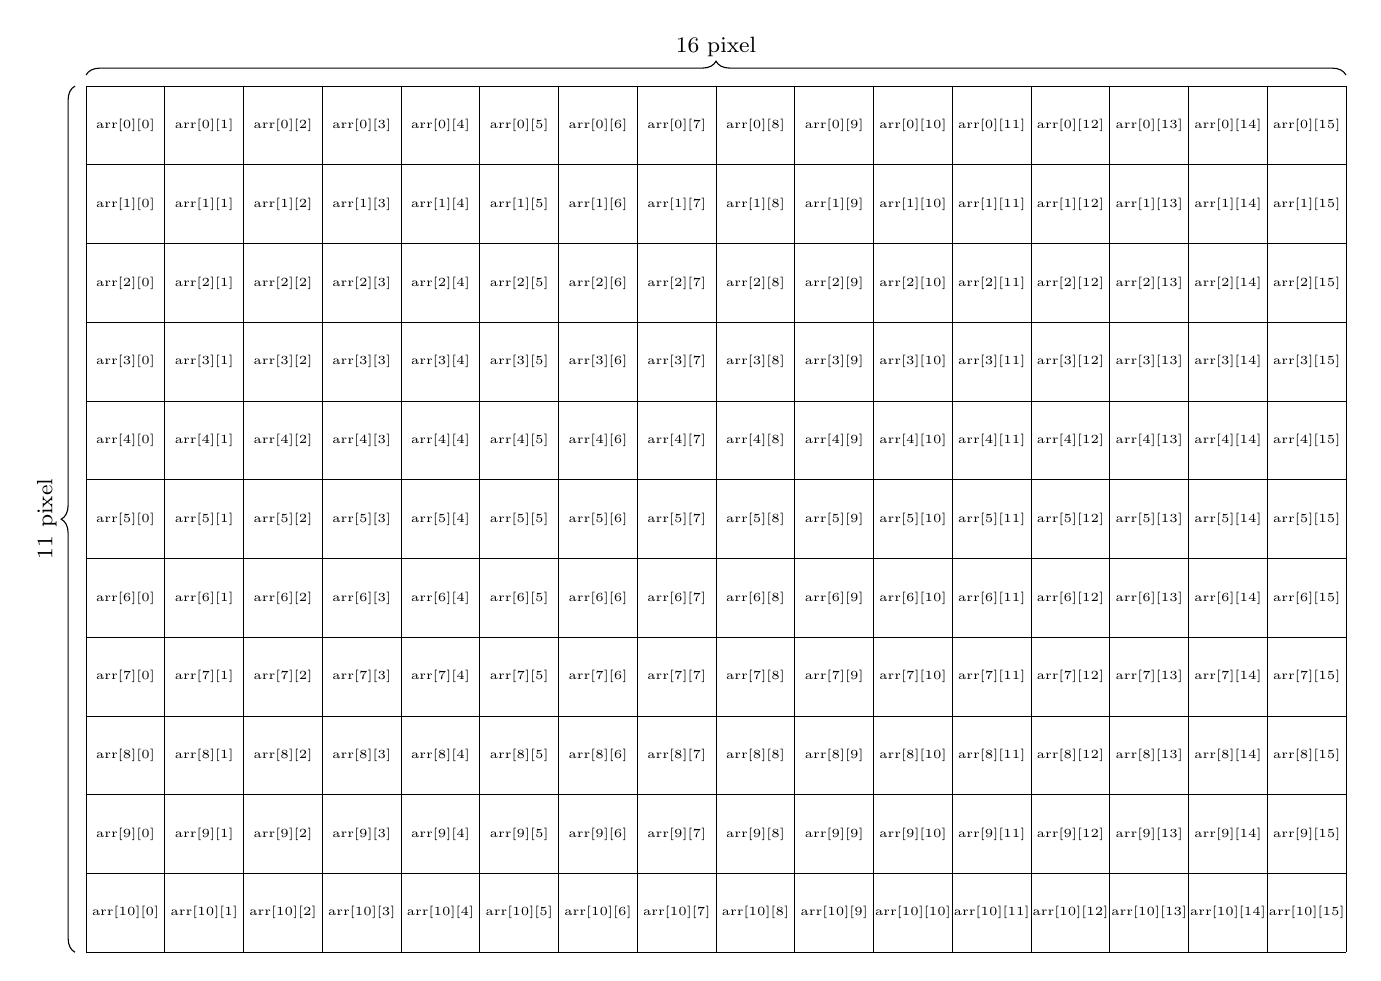
\begin{tikzpicture}

\draw [decorate,decoration={brace,amplitude=5pt,raise=4pt},yshift=0pt]
(-0.5,0.5) -- (15.5,0.5) node [black,midway,yshift=0.5cm ] {\footnotesize
	$16$ pixel};

\draw [decorate,decoration={brace,amplitude=5pt,mirror,raise=4pt},yshift=0pt]
(-0.5,0.5) -- (-0.5,-10.5) node [black,midway,xshift=-0.5cm,rotate = 90] {\footnotesize
	$11$ pixel};

  \begin{scope}
%\draw [step=0.03,very thin] (-1, 5.9) grid (-0.79, 6.26);

\foreach \row in {0,1, ..., 10}
{
	\foreach \col in {0, ..., 15}
	{
		\node[xshift=\col cm, yshift=-\row cm,font=\tiny,scale=0.9]
		{arr[\therowval][\col]};
		\stepcounter{somevalue}
	};
\stepcounter{rowval}
}


\foreach \r in {-0.5, ...,16}{
\draw [line width=0.1mm](\r, 0.5) -- (\r, -10.5);
}

\foreach \col in {-0.5, ..., 11}{
\draw [line width=0.1mm](-0.5,-\col) -- (15.5,-\col);
}
\end{scope}


\end{tikzpicture}
\end{document}
